\documentclass[11pt]{article}
\usepackage[T1]{fontenc}
\usepackage[utf8]{inputenc}
\usepackage[margin=1in]{geometry}
\usepackage{lmodern,microtype,amsmath,amssymb,booktabs,graphicx,tabularx}
\usepackage[round,authoryear]{natbib}
\usepackage[colorlinks=true,allcolors=blue]{hyperref}
\usepackage{placeins}
\graphicspath{{../../artifacts/verification_escalation/repair/figures/}}
\setlength{\parskip}{4pt}
\setlength{\parindent}{0pt}
\setlength{\emergencystretch}{2em}
\title{Executable Agreement and Clarification Demand in SQL Workflows}
\author{OverseeingManyLLMs research note}
\date{September 2026. Separate exploratory draft, not submitted.}
\begin{document}
\maketitle
\begin{abstract}
A user supervising several agents should not need to repeat information already available or resolve uncertainty that leaves the requested work unchanged. We implement a protocol that recovers scoped instructions, executes competing SQL interpretations, releases conditionally invariant table artifacts, and escalates remaining decisions. We test it against source recovery with minimum sufficient completion using a frozen, source-disjoint follow-up of 24 AMBROSIA databases and two generation/intent replicas. The requests and interpretation annotations are human-authored; the databases and new SQL proposals are generated. Verification uses 40 rather than 48 intent answers, but matching tables fall from 19 to 16 and mismatched releases increase from 22 to 26. Supplying all annotated alternatives eliminates every question saving. Controlled synthetic cases show when conditional release is sound and when correlated omissions make it harmful. The results support consequence displays and explicit verification boundaries, but not automatic question suppression from uncalibrated generated-candidate agreement.
\end{abstract}

\section{The decision problem}
A person managing several agents may face repeated questions, lost instructions and unfinished work that could proceed independently. Prior work in this repository found that additional clarification sometimes compensated for information lost during interpretation. It also found that a simple completion policy could match a deeper planner with fewer answers. These observations motivate a different process: recover available information first, test the consequences of remaining uncertainty, and ask only when a relevant distinction remains.

Our question is whether executable consequence checks can reduce substantive user decisions beyond a strong source-recovery and completion baseline while preserving useful outcomes. We distinguish four situations. A fact may be recoverable from an available instruction. Several meanings may remain but yield an invariant authorized artifact. The meanings may produce different artifacts and justify escalation. Finally, a task may remain unsupported because implementations or evidence are inadequate. The system must retain unfinished goals rather than manufacture savings by suppressing their questions.

This note contributes an executable, instrumented protocol and a paired evaluation of its failure boundary. It does not introduce minimax regret, information gathering, shared memory or a new scheduling optimizer. Its central empirical finding is negative: agreement among generated interpretations concealed omitted meanings. The existing submission and historical experiments remain separate.

\section{Relation to existing methods}
Generating alternatives is established in text-to-SQL. LogicalBeam diversifies plans and parses under schema ambiguity \citep{bhaskar-etal-2023-benchmarking}. AmbiSQL detects ambiguity, offers Other/Abstain, stores preferences and iteratively rewrites requests \citep{ding2026ambisql}. PRACTIQ already permits helpful outputs covering some alternatives without asking \citep{dong-etal-2025-practiq}. BIRD-Interact combines knowledge retrieval, execution feedback and interactive ambiguity resolution \citep{huo2026birdinteract}. Its reference SQL and tests still required a maintainer request at our access check, so we did not build the evaluation around them.

Execution-based comparison is also established. Disambiguate First, Parse Later compares SQL outputs to detect missing interpretations, trains an infiller and removes redundant results \citep{saparina-lapata-2025-disambiguate}. Sphinteract uses summarization, review, questions and early stopping, with actual participant evidence \citep{zhao2024sphinteract}. Most closely, SOMA-SQL combines multiple candidates, synthetic query-log retrieval and targeted execution probes to infer intent and repair SQL \citep{somayajula2026soma}. It is a preprint whose inspected paper provided prompts but no linked author implementation. We do not reproduce its system or claim that adding execution to retrieval is novel.

Value of Information explicitly weighs expected communication benefit against cost \citep{dong-etal-2026-value}. KnowNo uses calibrated prediction sets and requests help when alternatives remain \citep{ren2023knowno}. Our safeguards have no corresponding coverage guarantee. The potential distinction is narrower: a system may release an invariant \emph{artifact} while explicitly retaining uncertainty about meaning. A plausible pattern in a database does not authorize choosing a user's preference. The experiment tests whether this boundary is useful with fallible candidate generation.

\section{A bounded verification and escalation protocol}
Let $T$ be distinct user-valued deliverables. Task $j$ contains a public request, sources, a registered decision dependency, scope, exceptions, a version, a database snapshot $X_j$ and an output contract $K_j$. A source record distinguishes an explicit user requirement from an inference. A candidate set $C_j$ contains at most six SQL programs generated from permitted evidence. Evaluator references and the intended annotation are not controller inputs.

Define $E(c,X,K)$ as bounded read-only execution followed by contract-specific normalization. Its value is either a table or failure. We choose finite-set output agreement rather than a regret optimizer:
\begin{equation}
 \forall c\in C_j:\quad E(c,X_j,K_j)=R_j, \qquad E(c,X_j,K_j)\ne\mathrm{failure}.
 \label{eq:certificate}
\end{equation}
When public task constraints also permit snapshot output, $R_j$ is invariant over the represented set. This is a conditional certificate, not a guarantee that the correct interpretation belongs to $C_j$. It establishes neither universal SQL equivalence nor absolute semantic quality. It cannot override an explicit requirement to choose a meaning, follow a process or obtain authorization.

The protocol first attempts recovery from an available authoritative source with an exact citation, matching scope and no applicable exception. This validates provenance, not the generated SQL implementation. It then executes all candidates. Failed candidates block verification and are never discarded to manufacture consensus. In the generated condition, release additionally requires two generation passes, at least two distinct SQL strings, no declared unrepresented alternative, and a nonempty table. These development-fixed heuristics are not calibrated probabilities. Distinct strings may encode the same mistake, and a zero-valued aggregate is still a nonempty table.

If release is not supported, the controller exposes the candidate consequences, affected scope and work that can proceed without an answer. It asks a targeted intent question when the remaining budget permits. A received response is implemented separately for the relevant tasks. An unresolved response consumes its interaction unit and leaves the task unfinished. Shared answers apply only to registered dependencies with matching scope, version and exceptions. Similar wording alone does not establish shared authority.

The answer budget $B$ counts substantive intent responses, including unresolved replies. The demonstration counts a new scope restriction separately from its value answer. The machine budget $M$ counts SQL executions, including failures. Model calls are separately recorded. Counters are checked and charged before operations, so every executed path satisfies its limits. Cache keys include the represented source, request, contract, scope, version, candidates and snapshot. Changes invalidate the corresponding artifact. These properties cover registered dependencies, not unknown semantic relationships.

\subsection{Output and computation boundaries}
We score snapshot tables rather than reusable programs. Normalization preserves column position, width, duplicate row multiplicity, NULL and exact normalized numeric/text values. Aliases are ignored. Explicitly requested sorting is detected from released text before generation and row order is then preserved. The detector is finite and may miss unfamiliar phrasing. Unordered tables use bags of rows. The source benchmark's unordered comparator flattens cell values across rows; we use the stricter declared contract instead.

SQLite execution is read-only, limited to 100,000 virtual-machine instructions and 500 rows. Each empirical task receives at most 24 executions. One inspection uses at most six candidate checks, with memoization. The frozen terminal controller can retry an unchanged failed answered query on a later inspection; these executions remain charged. The online wrapper caches that failure. Model preparation is not free even when a replay does not consume an answer branch.

The descriptive loss is
\begin{equation}
 L=4\sum_j \mathbf{1}[j\text{ released a mismatched table}]
   +\sum_j \mathbf{1}[j\text{ unfinished}].
\end{equation}
These dimensionless weights are constructed assumptions. We report answer demand, table agreement, mismatched releases, unfinished work and computation separately. No claim of noninferiority or measured cognitive-load reduction follows from this score.

\section{Data, freeze and comparisons}
\subsection{An externally authored ambiguity benchmark}
AMBROSIA contains human-authored ambiguous requests and disambiguated interpretations over generated, author-filtered databases \citep{saparina2024ambrosia}. Scope and attachment SQL uses templates, while vague-query SQL is human-authored. The source is not observed production activity. Its public assets support executable reference comparison, unlike the unavailable BIRD-Interact reference package. It contains no annotated shared decision across our separate source tasks.

Nine databases supported two development passes. A first frozen 48-database evaluation exposed a concrete adapter defect: its blanket unordered contract and prompt contradicted two explicit ranking requests. Those outcomes are preserved as a flawed-adapter diagnostic. They are not pooled into the ordering-correct follow-up or retroactively repaired by rescoring.

Before new generation, a second commit froze the public ordering contract and 24 disjoint test databases, eight per ambiguity type, excluding all 57 earlier databases. Source order and the existing eligibility rules fixed selection before outcomes. No method or utility tuning followed. The fresh requests contain no detected explicit sorting, so ordering correctness is tested semantically in focused tests, not estimated as an empirical treatment effect.

Each database has two generation/intent replicas. Public sampling seeds vary, and a fixed hash rotates the selected source annotation. These replicas combine generation and intent variation. They are averaged within database before paired analysis. The 24 databases span four domains and shared source construction conventions, so source-level intervals do not establish broad-population independence. The sample deliberately contains ambiguity and cannot estimate its prevalence in ordinary agent work.

\subsection{Generated, privileged and source-availability conditions}
The primary condition generates up to three interpretations in each of two public passes. A separate cached model response implements the simulated user's annotated clarification. It is inaccessible until a policy asks. The simulator supplies a correct intent annotation even if the displayed candidate set is inadequate; actual humans might not understand or correct such a question. The subsequent SQL implementation can still fail.

A privileged diagnostic supplies all reference SQL alternatives and an exact returned implementation. It isolates consequence checking from candidate and answer implementation failures. A source-availability diagnostic on six of the same databases places the relevant human-written clarification in an existing scoped instruction. This is an authored availability manipulation, not an original multi-turn dialogue. It is a paired subset, not six new independent cases.

The existing Qwen2.5-7B-Instruct model ran serially in BF16 on one RTX 6000 Ada with no CPU offloading. Revision and tokenizer revision were \texttt{a09a35458c702b33eeacc393d103063234e8bc28}. Temperature was 0.3, top-p 1, context 2,048 tokens and output limits 512 for candidates and 256 for answered SQL. All methods reuse the same saved preparations and response branches. The corrected batch requires 156 generations and 3,240 policy/condition rows. No new calls are needed for scheduling or policy replay.

\subsection{Baselines and analysis}
Recovery plus minimum sufficient completion and recovery plus the previous two-step planner share the same evidence, candidates, release constraints and abstract utility. Each source task has one unresolved intent represented by an assumed equiprobable binary factor with error weight four and deferral weight one. They therefore make the same question decision here. They do not know an unasked annotation. Full-context answering releases the first executable candidate. Matched checking selects the modal execution result. These are controlled adaptations, not full reproductions of published agents.

Ablations remove source recovery, verification, coverage guards, sharing or selective continuation. Budgets are zero, one and two. The primary contrast is verification minus recovery/completion at budget one, reported for each outcome component. We average replicas within source database, then use 2,000 paired bootstrap resamples with fixed seed 86421. Failed and unfinished tasks remain in the denominator. All policies and replicas for a source stay together. Loss sensitivity uses mismatch weights one, two, four and eight on unchanged trajectories.

\section{Results and diagnosis}
\begin{table}[ht]
\centering\small
\caption{Corrected generated-candidate condition, 24 source databases and 48 replicas, budget one. Human-authored reference annotations score generated SQL on generated databases. Answers and policy outcomes are simulated. Loss is $4\times$ mismatch $+$ unfinished. These are frozen outputs before the post hoc integrity quarantine discussed below.}
\label{tab:main}
\begin{tabular}{lrrrrr}
\toprule
Method & Answers & Match & Mismatch & Unfinished & Loss \\
\midrule
Recovery + completion & 48 & 19 & 22 & 7 & 95 \\
Recovery + depth two & 48 & 19 & 22 & 7 & 95 \\
Verification & 40 & 16 & 26 & 6 & 110 \\
Full-context proposal & 3 & 14 & 34 & 0 & 136 \\
Matched checking & 3 & 14 & 34 & 0 & 136 \\
No coverage guard & 40 & 16 & 26 & 6 & 110 \\
\bottomrule
\end{tabular}

\end{table}
Verification reduces answers from 48 to 40, but matching tables fall from 19 to 16 and mismatched releases rise from 22 to 26 (Table~\ref{tab:main}). One additional task is released rather than left unfinished, but its table mismatches. Loss increases from 95 to 110. At source level, verification wins on no database, ties on 20 and loses on four.

The mean answer difference is $-0.1667$ per task, with paired 95\% interval $[-0.2708,-0.0625]$. Matching tables change by $-0.0625$ $[-0.1458,0]$, mismatched releases by $+0.0833$ $[+0.0208,+0.1667]$, and unfinished work by $-0.0208$ $[-0.0625,0]$. The loss difference is $+0.3125$ $[+0.0625,+0.6250]$. These results do not establish quality-preserving demand reduction. The small source-order sample and common construction conventions remain important limits on the intervals.

\begin{figure}[ht]
\centering
\includegraphics[width=\linewidth]{quality_vs_questions.pdf}
\caption{Task outcomes versus simulated answer demand. Human-authored requests/annotations, generated databases and Qwen proposals, and replayed policy decisions. Bars are 95\% source-database bootstrap intervals with replicas averaged first. The right panel is a constructed source-availability subset. Its direct-reading star is a secondary prompt-style diagnostic. Less interaction does not imply acceptable task quality.}
\label{fig:quality}
\end{figure}

\subsection{Apparent savings arise from missing interpretations}
The generated sets cover the selected reference output in 15 of 48 replicas and every annotated output in none. Eight questions are suppressed. Six suppressed releases mismatch the target, and all six omit its output. There are 28 failed executions among 187 public candidates. The guard prevents failed candidates from creating agreement, but does not detect a missing successful interpretation. Removing the guard has no outcome effect in this corrected set.

In the privileged diagnostic, all 24 databases have different reference outputs across their interpretations. Both completion and verification ask 48 questions and return 48 matching tables. Thus no source-supported harmless-ambiguity region appears in this sample. The two generated suppressions that match the selected intent still omit another supported interpretation. Their current correctness is not evidence of complete coverage.

Reference-table mismatch is not synonymous with semantic error. Developer inspection found one of the six suppressed mismatches attributable solely to extra projected columns. Five involve a missing semantic requirement. The four incremental mismatches relative to completion involve attachment, collective scope or inclusive interpretations, rather than projection alone. This post hoc code inspection is not an independent expert study or a replacement scoring metric.

\begin{figure}[ht]
\centering
\includegraphics[width=\linewidth]{paired_differences.pdf}
\caption{Matched corrected-study outcomes. Left: mean replica loss difference for each source database; negative would favor verification. Right: outcome component differences with paired source-level intervals. Quantities are generated/executed task outcomes under a simulated answer budget and declared loss, not observed human performance.}
\end{figure}

\subsection{Recovery is the more useful opportunity}
In the six-database availability subset, exact source provenance is recovered for seven of 12 preparations. Completion uses five answers and returns five matching, six mismatched and one unfinished result. Verification uses four answers and returns four matching, seven mismatched and one unfinished result. Its additional suppression loses a matching result.

A secondary direct-reading diagnostic uses the cached SQL response to the exact same available instruction with no extra question. It returns the same five matching, six mismatched and one unfinished result as completion. This changes prompt style and is reported separately from the frozen common-backend comparison. It demonstrates that repeated questions can compensate for an unnecessarily narrow recovery interface. It does not solve the remaining implementation failures.

Full-context first-executable release and modal checking use three questions but produce 34 mismatched releases each. They save more demand by accepting more errors. At budget zero, completion leaves 48 tasks unfinished; verification releases two matching and six mismatched tables and leaves 40 unfinished. Budget two repeats budget one because the adapter offers only one intent response per task.

The mean loss difference remains nonnegative at every declared mismatch weight: $+0.0625$, $+0.1458$, $+0.3125$ and $+0.6458$ for weights one, two, four and eight. This is sensitivity rescoring, not evidence for a utility-adapted controller. A post hoc four-domain aggregation also remains unfavorable but is too small for stable generalization.

\subsection{Source integrity limits the frozen release rule}
The source metadata records foreign-key violations in four selected databases. All 56 reference queries execute, but successful execution is insufficient validation of source integrity. The frozen rule did not gate releases on these violations. One of its eight agreement releases occurs on an affected database. The current online prototype adds a public, budgeted integrity guard and leaves affected goals unfinished.

A post hoc uniform-quarantine sensitivity retains all 24 source units and blocks both replicas of those four databases for every policy. Completion then uses 40 answers, with 17 matching, 18 mismatched and 13 unfinished results. Verification uses 33 answers, with 14 matching, 21 mismatched and 13 unfinished results. Loss changes from 85 to 97. The paired difference is $+0.25$ with interval $[0,0.50]$, and zero wins, 21 ties and three losses. The adverse point estimate persists, but the interval includes zero. This is saved-output sensitivity on inspected cases, not a new guarded evaluation or a new timing measurement. The original rows remain unchanged.

\subsection{A post hoc direct-reading audit}
The primary full-context control takes the first executable candidate from an interpretation-enumeration prompt. After inspecting the principal result, we declared a separate direct-reading, answer-or-ask prompt on four fixed development cases and both replicas of the same 24 source databases. Its 52 calls were committed before generation. This is a post hoc comparator audit on already inspected cases, not a fresh held-out evaluation. No primary method, sample or outcome changed.

The direct reader declares 42 replicas ready and asks in six. At budget one it returns 12 matching, 30 mismatched and six unfinished results, with loss 126 and 48 SQL executions. None of its six clarification branches yields a matching table. A failed query remains unfinished rather than asking the user merely to fix syntax. This simpler prompt does not solve the ambiguity problem. It remains distinct from direct reading in the source-availability condition, where an explicit prior instruction permits zero additional questions with the completion baseline's outcome counts.

\subsection{Concrete matched cases}
The frozen rule selects the first lexicographic source ID by favorable, tied or unfavorable mean loss, retaining both replicas. No favorable empirical loss case exists. ID 1475 is a tie. Both methods ask, one clarified implementation misses the common-to-all requirement, and the other replica matches. ID 1484 is unfavorable. In one replica the intended output is the program common to all authorities. Generated candidates instead agree on the authority/program join. Verification releases six rows without asking; completion asks and returns the one-row common-program result. Both methods match the other replica.

\section{Synthetic mechanisms and the working desk}
Seventeen authored family labels with 16 nuisance seeds, three budgets and ten methods produce 8,160 controlled rows. These are not 272 independent observations of real work. Some labels repeat a structure. A supplied complete pair of interpretations yielding the same IDs lets verification save an answer while preserving the table. Different outputs require a question. An explicit semantic-choice contract also requires an answer even when outputs agree. Missing intended candidates and correlated wrong interpretations produce incorrect releases without questions. Failed queries and direct empty-result traps block verification.

A registered exception does not inherit another scope's answer. A count can nevertheless proceed independently when it is invariant. In the authored three-goal workload, verification releases the count and inventory before an export decision. At budget zero, global waiting releases neither; at budget one, both methods finish all goals. This models independent progress, not human reading time. The no-sharing ablation often ties because the count already agrees across interpretations. A separate online test repairs a duplicate-question guard for two consequential tasks, but provides no new empirical sharing benefit.

Changed snapshots invalidate earlier certificates. The nonempty check has a clear limit: two wrong COUNT queries can return the same zero-valued row. The final boundary tests preserve this failure. No amount of agreement within an incomplete set proves that the actual meaning is included.

\begin{figure}[ht]
\centering
\includegraphics[width=\linewidth]{synthetic_ablations.pdf}
\caption{Authored synthetic arithmetic at budget one, compared with recovery/completion. Numbers are mean differences across nuisance seeds, not estimated human effects. Supplied interpretations, shared dependencies, failures and snapshots are constructed. Favorable equality cases and harmful omissions are shown together. The no-sharing ties partly reflect an invariant count and should not be interpreted as a general finding about sharing.}
\end{figure}

The local Decision desk exposes scoped sources, ready and unfinished goals, competing outcomes, affected work and remaining answer/check budgets. It supports broad or narrow answers, unresolved replies, revised definitions and changed data. A revision leaves unrelated goals ready. A narrow scope choice consumes an additional answer unit. Technical evidence is expandable rather than placed in the main decision card. Fourteen browser checks and 18 displayed interactions were recorded and replayed. They are scripted software observations, not participant data.

\section{Interpretation and next step}
The protocol provides a practical distinction between recovering an instruction, conditionally releasing a table and asking about meaning. However, generated agreement does not establish that a consequential interpretation is absent. In this experiment, the safer savings came from direct source reading. The generated-candidate mechanism lowered answer counts at the expense of the declared outcome contract.

The evidence does not establish an empirical advantage specific to many agents. Source tasks lack annotated shared decisions, and a single orchestrator could run this controller. Shared scope and selective continuation are demonstrated only in explicitly authored workloads. There is no measurement of mental demand, frustration, human response accuracy or operational financial loss.

The strongest defensible research result is an auditable negative finding about candidate omission at a conditional verification boundary. It is not a new general algorithm for communication or an advantage over the closest published systems. We recommend source recovery and targeted clarification as the default. Automatic suppression should be restricted to interpretation sets justified independently of uncalibrated model agreement. Before making this the paper's central contribution, a new study needs source-grounded shared decisions, independently defined acceptance contracts, better candidate coverage and actual interaction observations. Simply expanding this timing-free replay matrix would not supply that evidence.

\section{Reproducibility and preservation}
The package records public asset revisions and checksums, split exclusions, both protocol freezes, generated SQL, attempts, source hashes, complete policy outcomes and plotting code. Source data and raw prompt envelopes remain local and excluded from Git in accordance with the AMBROSIA authors' request against dataset uploads. A clean checkout reconstructs source inputs from the original public download and replays the committed derived outputs. This redaction decision is explicit and does not alter historical publication records. Source disjointness is within this project, not evidence that the model's training data excluded the public benchmark.

The session scheduled 592 model calls and made 586 GPU attempts. Six development calls exceeded the context limit before generation. There were no transport retries or failed GPU attempts, and two successful responses were unparseable. Total usage was 461,283 prompt and 79,978 completion tokens. Summed generation latency was 1,673.44 seconds. This is not provider billing time. Controller median time was 2.48 ms for verification and 2.79 ms for completion in the primary condition. Both include measured CPU execution, while model preparation is accounted separately.

Thirty-four focused tests and 27 relevant historical regression tests passed. Saved-output replay matches all 3,240 corrected rows, 6,480 initial diagnostic rows and 8,160 synthetic rows, their event traces and the eight primary analysis tables. Another 144 post hoc direct-reader rows and their paired analysis replay separately. Historical trajectories, clocks and the submission manuscript are preserved. New work has its own three-hour authorization; it is not described as occurring within the expired original 36-hour window. Final elapsed and cumulative accounting accompany the repository report.

\FloatBarrier
\bibliographystyle{plainnat}
\bibliography{../../research/verification_escalation/references}

\clearpage
\appendix
\section{Additional visual diagnostics}
\begin{figure}[ht]
\centering
\includegraphics[width=\linewidth]{coverage_and_cost.pdf}
\caption{Generated-candidate diagnostics on the corrected source set. Reference-output coverage is evaluator-only and weaker than semantic coverage. SQL executions and simulated answers are recorded separately. All compared methods reuse the same preparation calls. These costs are not human workload measurements.}
\end{figure}
\begin{figure}[ht]
\centering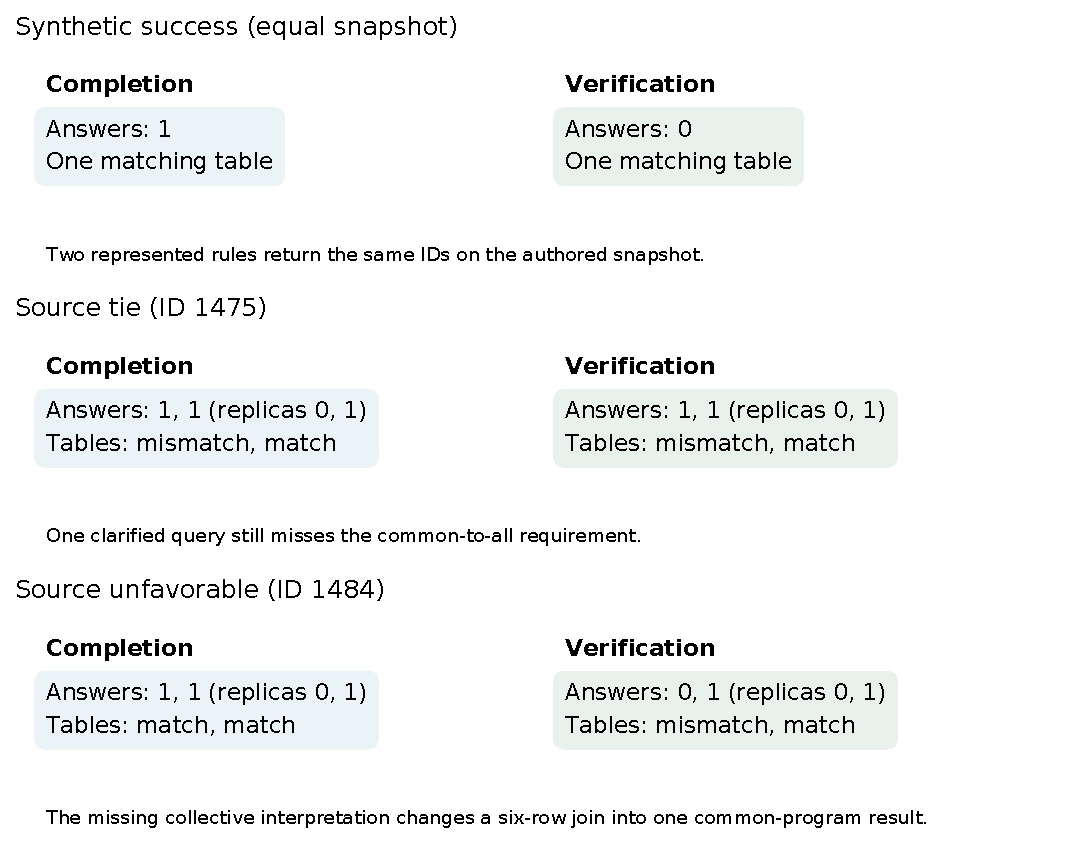
\includegraphics[width=\linewidth]{matched_examples.pdf}
\caption{A constructed equality success and the frozen first tied/unfavorable empirical source IDs. Both empirical replicas are retained. Questions are simulated and outputs are generated/executed. No favorable empirical loss example was available; it is not replaced by a selectively chosen one.}
\end{figure}
\begin{figure}[ht]
\centering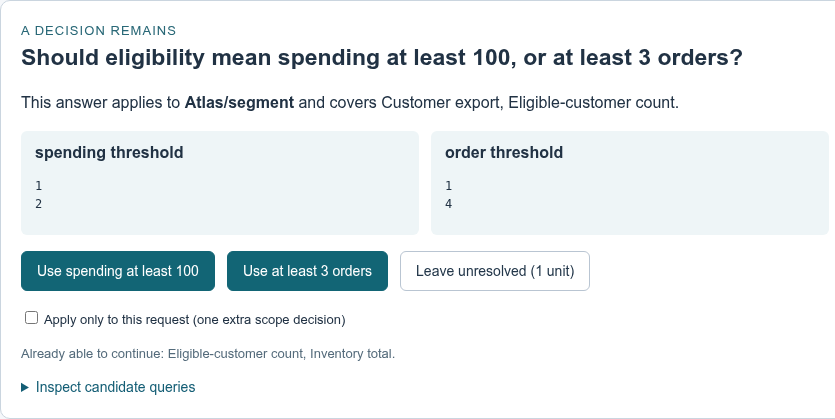
\includegraphics[width=.95\linewidth]{../../artifacts/verification_escalation/interface/final/paper_question.png}
\caption{The working local desk on authored analytics data. It presents the scope, differing customer IDs and already available count/inventory. The full interface separately tracks budgets. The screenshot is a scripted demonstration, not evidence of human decision quality or cognitive load.}
\end{figure}
\end{document}
